%% bare_conf.tex
%% V1.3
%% 2007/01/11
%% by Michael Shell
%% See:
%% http://www.michaelshell.org/
%% for current contact information.
%%
%% This is a skeleton file demonstrating the use of IEEEtran.cls
%% (requires IEEEtran.cls version 1.7 or later) with an IEEE conference paper.
%%
%% Support sites:
%% http://www.michaelshell.org/tex/ieeetran/
%% http://www.ctan.org/tex-archive/macros/latex/contrib/IEEEtran/
%% and
%% http://www.ieee.org/
\documentclass[11pt,conference]{IEEEtran}
\usepackage{blindtext, graphicx}
\usepackage{algorithm}
\usepackage[noend]{algpseudocode}
\usepackage[font=footnotesize,labelfont=bf]{caption}
\usepackage{placeins}
\usepackage[cmex10]{amsmath}
\usepackage{cite}
\usepackage{array}
\usepackage{mdwmath}
\usepackage{mdwtab}

% correct bad hyphenation here
\hyphenation{op-tical net-works semi-conduc-tor}


\begin{document}
%
% paper title
% can use linebreaks \\ within to get better formatting as desired
\title{Adaptive Write-Update and Write-Invalidate Cache Coherence Protocols for Producer-Consumer Sharing}


% author names and affiliations
% use a multiple column layout for up to three different
% affiliations
\author{\IEEEauthorblockN{Bangjie Liu}
\IEEEauthorblockA{Language Technologies Institute\\
School of Computer Science\\
Carnegie Mellon University\\
\texttt{bangjiel@andrew.cmu.edu}}
\and
\IEEEauthorblockN{Hao Li}
\IEEEauthorblockA{Language Technologies Institute\\
School of Computer Science\\
Carnegie Mellon University\\
\texttt{haol2@andrew.cmu.edu}}
}

% make the title area
\maketitle


\begin{abstract}
Shared memory multicore systems play crucial roles in scientific and enterprise applications. They are efficient in general applications but perform poorly in applications that establish producer-consumer sharing patterns under write-invalidate cache coherence protocol due to a large amount of cache invalidations and cache misses. Write-update protocol mitigates this issue by forwarding all updates on write operations but introduces extra network traffic overhead. In this project, we propose an adaptive cache coherence protocol that speculatively forwards data updated by producer to potential consumers when producer-consumer sharing patterns are detected to avoid unnecessary invalidations and memory accesses. We evaluate the proposed adaptive protocol on applications with varying degree of producer-consumer sharing patterns. As a result, it outperforms write-invalidate protocol by 2\% --- 21\%.
\end{abstract}


\section{Introduction}
Shared memory multicore systems play increasingly important roles in both scientific world and the industry. Cache coherence protocol has great influence on performance of shared memory multicore systems. Producer-consumer sharing refers to situations in multi-process synchronization wherein multiple processes share a common, fixed-size buffer and some processes, as known as producers, keep writing new data to that shared buffer while some readers keep reading data from it \cite{wiki}. The most popular cache coherence protocol used in modern multiprocessor architecture is directory-based write-invalidate protocol, which is inefficient for producer-consumer sharing due to extensive invalidation traffics and expensive remote misses.

Researches have been done in this area, but they focus more on eliminating unnecessary hops as shown in Figure \ref{write_invalidate_hops} by using a naive pattern detector and additional hardware for cache directory \cite{work1}.
\begin{figure}[!h]
\centering
\captionsetup{justification=centering}
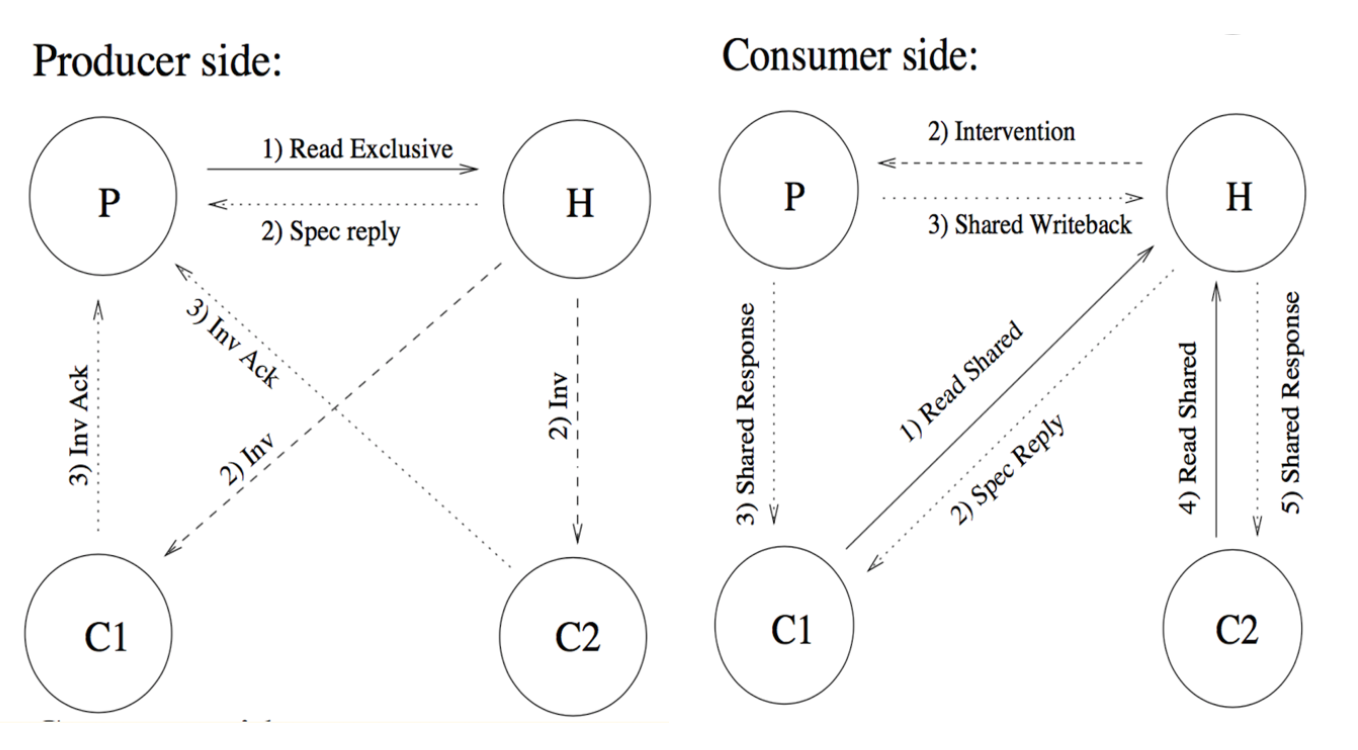
\includegraphics[width=3.5in,height=1.8in]{write_invalidate_hops.png}
\caption{Producer-Consumer Remote Misses}
\label{write_invalidate_hops}
\end{figure}
\FloatBarrier

 Instead of mitigating remote misses, this project focuses on mitigate the slowest part --- memory accesses caused by invalidation. It assumes that communications among caches on different cores are physically feasible and contributes to the following:
\begin{itemize}
  \item A sophisticated detector that detects producer-consumer sharing patterns at a fine-grained level without extra hardware
  \item An adaptive cache coherence protocol optimized for producer-consumer sharing patterns
\end{itemize}

The remainder of this report is organized as follows. We start in Section 2 with an overview of our goals and what we have accomplished. Section 3 describes our analysis of the performance of write-invalidate and write-update protocols on a representative producer-consumer application. In Section 4, we present our adaptive protocol, followed by a thorough evaluation on several applications in Section 5. Finally, we summarize our works and discuss future directions in Section 6 and 7.


\section{Goals}

\textbf{[75\%]} Implement cache simulators and testing tools (stack trace, logger, etc.) to fully evaluate and analyze the performance of directory-based write-invalidate and write-update protocols on representative multi-threaded producer-consumer applications.

\textbf{[100\%]} Implement proposed adaptive cache coherence protocols and producer-consumer sharing pattern detector. Evaluate and analyze the its performance on applications with varying degree of producer-consumer sharing.

\textbf{[125\%]} Equip the cache simulator with functionalities that can synchronize application threads so as to observe more accurate cache access events (mitigate the effect of pintool instrumentation).

As we write this report, we have accomplished both 75\% and 100\% goals. And due to time limits, we decide to work on a more thorough analysis of the proposed protocol on benchmarks with varying degree of producer-consumer sharing patterns instead of the 125\% goal.


\section{Write-Invalidate and Write-Update Protocols Evaluation}
In this section, we evaluate the performance, in terms of load/store hit rates, of write-invalidate and write-update protocols on a representative application that establishes producer-consumer sharing pattern. In the following evaluations, there are 1 producer and 2 consumers running on different cores. It is done on a Intel(R) Xeon(R) CPU E5-1660 v4 @ 3.20GHz machine with 32KB L1 data cache. And we only simulate L1 data cache configured as Table \ref{l1_cache_config_1}.

\begin{table}[!h]
\renewcommand{\arraystretch}{2.5}
\caption{L1 Cache Configuration}
\label{l1_cache_config_1}
\centering
\begin{tabular}{|c|c|c|c|}
\hline
Number of Sets & Associativity & Line Size & Interconnect \\
\hline
64 & 8 & 64B & Directory \\
\hline
\end{tabular}
\end{table}
\FloatBarrier

\subsection{Representative Application}
In the application, there is a producer thread that keeps writing to a shared memory while there are multiple consumer threads reading for it. They use a global lock for synchronization as shown in Algorithm \ref{producer_thread} and \ref{consumer_thread}. A such self-defined application works well for evaluation purposes because it offers overall performance evaluation under different cache coherence protocols. And more importantly we can have a fine-grained investigation of shared data of interest by outputting its memory address and look that up among all access records.

\begin{algorithm}
\caption{Producer Thread}
\label{producer_thread}
\begin{algorithmic}[1]
\State $data$ refers to a shared memory location
\State $lock$ refers to the lock for $data$
\While{True}
    \State GetLock($lock$) \Comment{get global lock}
    \State Produce($data$)
\EndWhile
\end{algorithmic}
\end{algorithm}

\begin{algorithm}
\caption{Consumer Thread}
\label{consumer_thread}
\begin{algorithmic}[1]
\State $data$ refers to a shared memory location
\State $lock$ refers to the lock for $data$
\While{True}
    \State GetLock($lock$) \Comment{get global lock}
    \State Consume($data$)
\EndWhile
\end{algorithmic}
\end{algorithm}


\subsection{Write-Invalidate Performance}
Write-invalidate protocol works poorly on producer-consumer sharing patterns. As Figure \ref{write_invalidate} indicates, the overall load hit rate is acceptable. But for the shared data alone as shown in Figure \ref{write_invalidate_1}, consumers' load hit rates are relatively low. The reason is that in write-invalidate protocol, write operations will invalidate all copies of this particular cache line and thus read operations after that need to read the latest one from either the owner or memory.

\begin{figure}[!h]
\centering
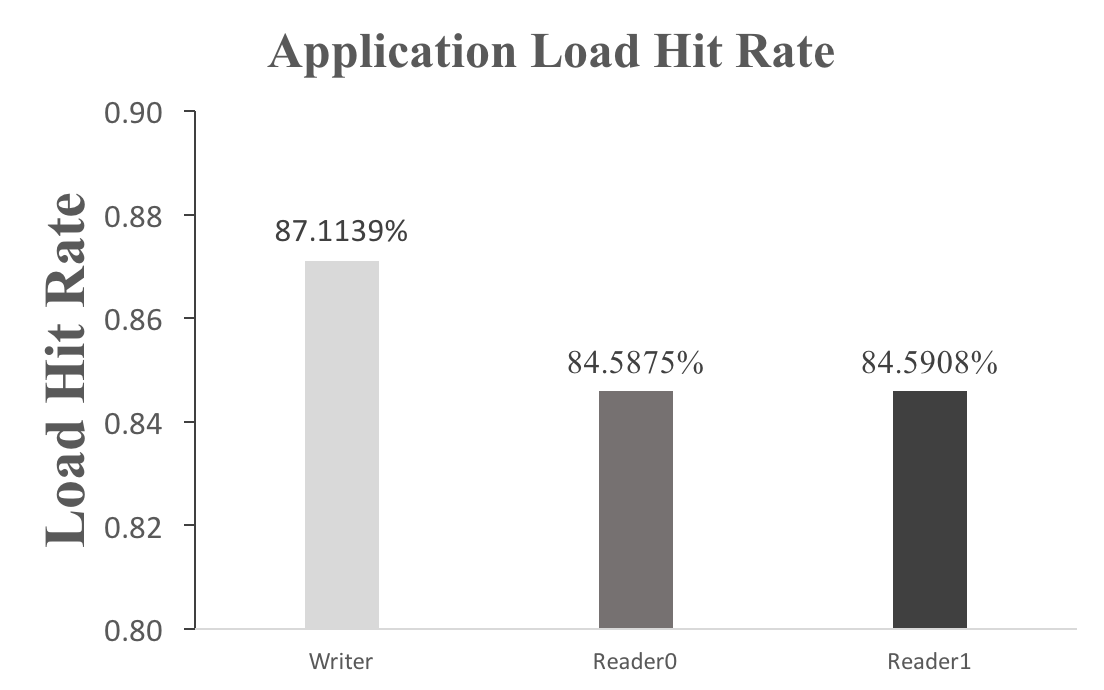
\includegraphics[width=3.2in]{write_invalidate.png}
\caption{Write-Invalidate Overall Load Hit Rates}
\label{write_invalidate}
\end{figure}
\FloatBarrier

\begin{figure}[!h]
\centering
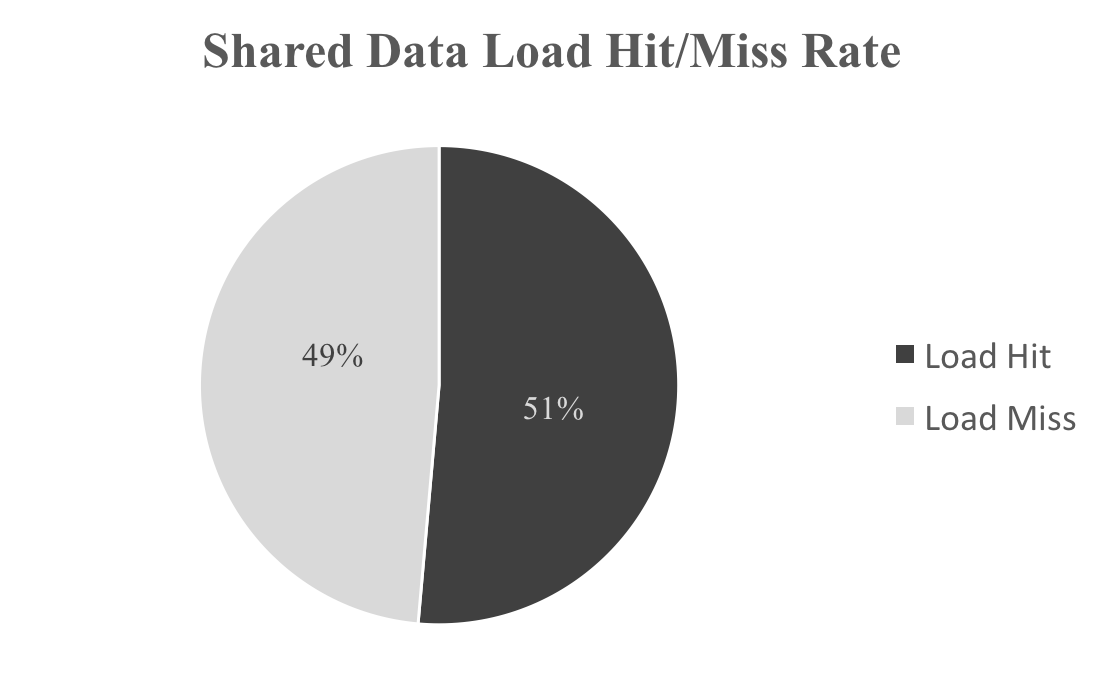
\includegraphics[width=3.2in]{write_invalidate_1.png}
\caption{Write-Invalidate Shared Data Load Hit Rates}
\label{write_invalidate_1}
\end{figure}
\FloatBarrier


\subsection{Write-Update Performance}
Write-update works well on producer-consumer sharing patterns. As Figure \ref{write_update} and \ref{write_update_1} shows, the overall performance is good and consumers have perfect load hit rates. This is because consumers now can directly get data from producer without accessing memory.

\begin{figure}[!h]
\centering
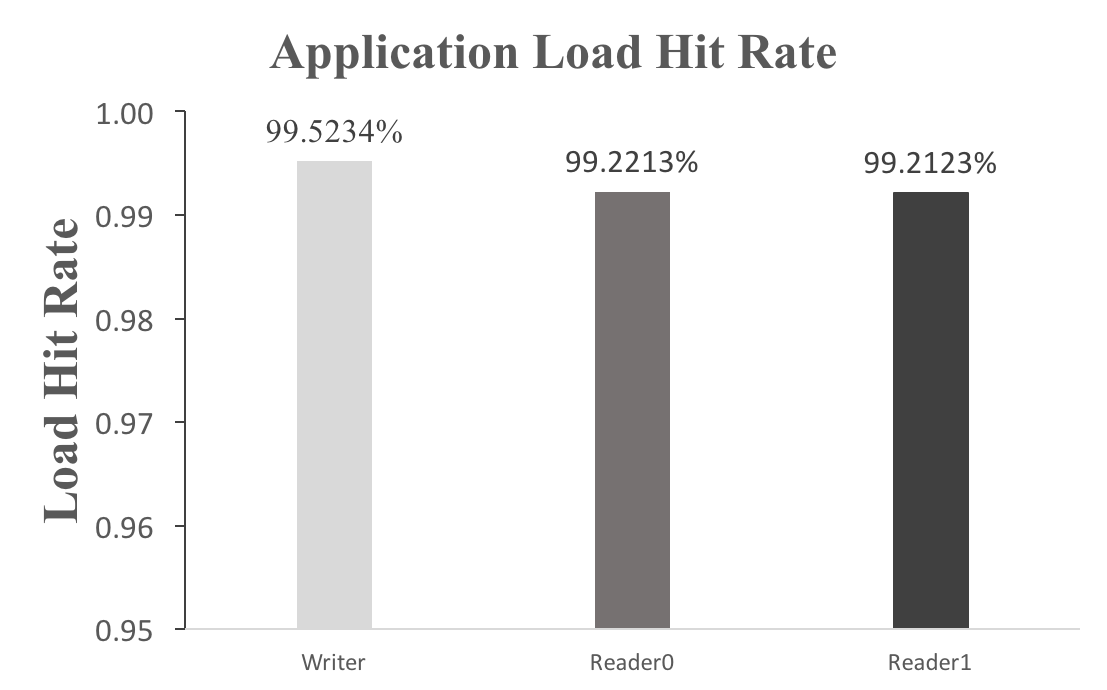
\includegraphics[width=3.2in]{write_update.png}
\caption{Write-Invalidate Performance}
\label{write_update}
\end{figure}
\FloatBarrier

\begin{figure}[!h]
\centering
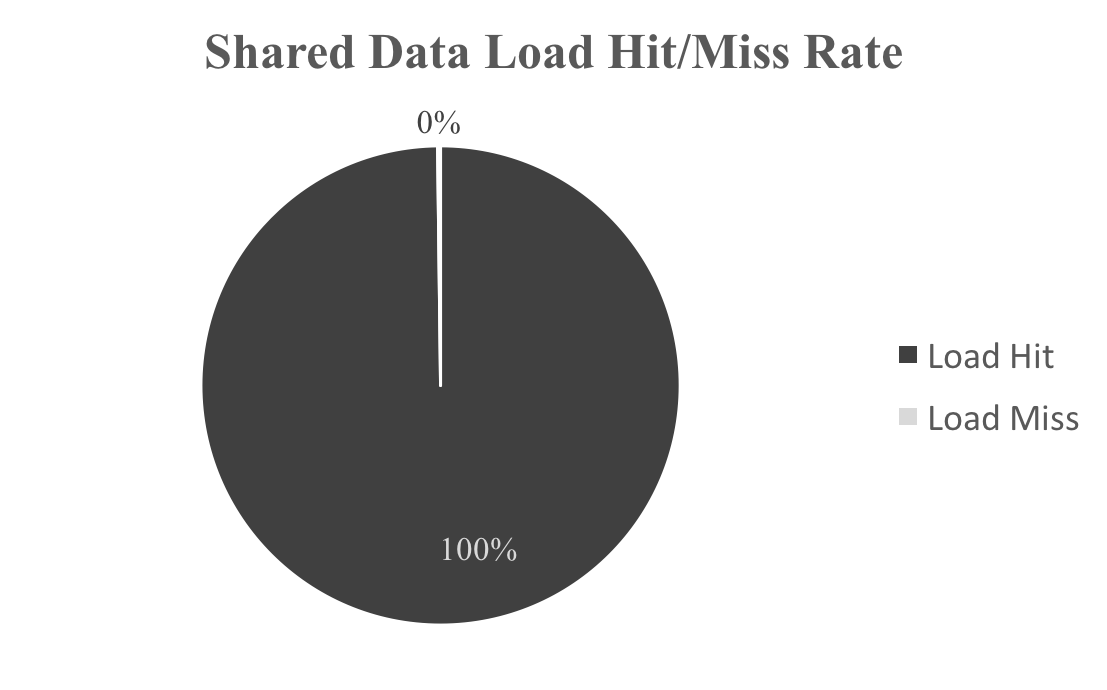
\includegraphics[width=3.2in]{write_update_1.png}
\caption{Write-Invalidate Performance}
\label{write_update_1}
\end{figure}
\FloatBarrier


\section{Adaptive Cache Coherence Protocol}
In this section, we introduce an adaptive cache coherence protocol that intelligently switches between write-invalidate and write-update protocols. It can mitigate unnecessary memory accesses by speculatively forwarding data to consumers once producer-consumer patterns are detected. Producer-consumer sharing patterns are defined as such: when a thread reads a memory location more than once after a thread writes it, the reading thread is considered as one of the consumers of the writing thread for this particular memory location.


\subsection{Detector}

Additional bits are needed to track access history of each cache line for pattern identification. They are associated with directory lines which are extended to the structure shown in Figure \ref{dir_line}.

\begin{figure}[!h]
\centering
\captionsetup{justification=centering}
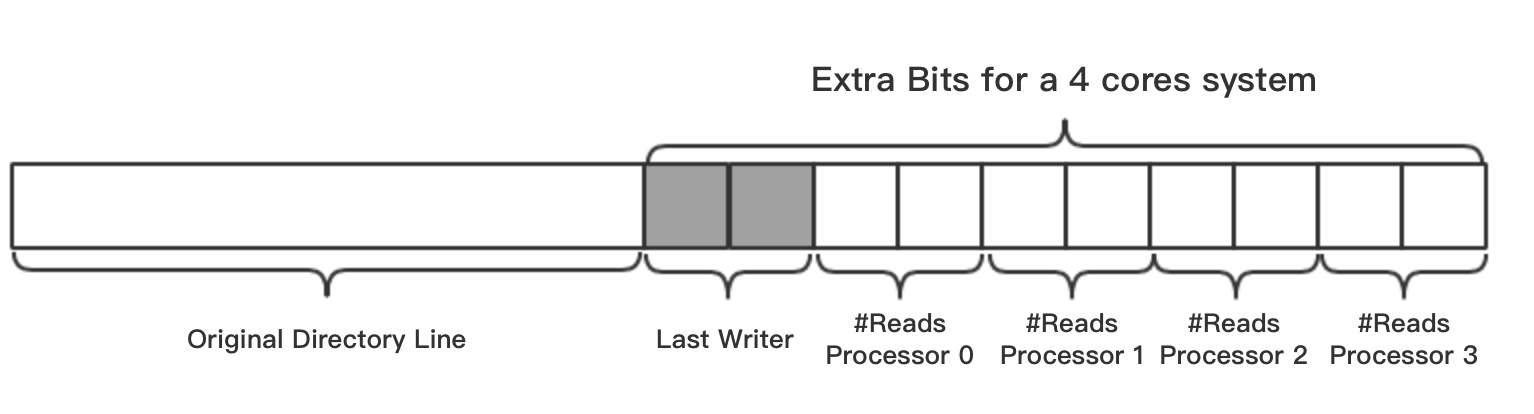
\includegraphics[width=3.5in]{dir_line.png}
\caption{Extended Directory Line Structure of a 4 Core Machine}
\label{dir_line}
\end{figure}
\FloatBarrier

The number of extra bits for each cache line is
\begin{equation*}
log N + 2 * N
\end{equation*}
where $N$ is the number of processors, $last\_writer$ tracks the last one to write this cache line, and there are 2 saturating bits for every processor to track the number of read operations on this cache line. Cache accesses will trigger updates on the extra bits as shown in Algorithm \ref{write_operations} and \ref{read_operations}. Note that the extra bits will be discarded to save space when its associated directory line is evicted. However, as mentioned in Section 1, we assume large enough directory banks for all line records and so have not simulate the eviction of directory lines.

\begin{algorithm}
\caption{On Read Operations}
\label{read_operations}
\begin{algorithmic}[1]
\State Let $pid$ refer to a processor
\ForAll{$pid$}
    \State SaturatingIncrease($pid$) \Comment{increase by 1}
\EndFor
\end{algorithmic}
\end{algorithm}
\FloatBarrier

\begin{algorithm}
\caption{On Write Operations}
\label{write_operations}
\begin{algorithmic}[1]
\State Let $writer\_id$ be the processor performing writes
\If{$writer\_id$ == $last\_writer$}
    \ForAll{$pid \neq writer\_id$} \Comment{exclude itself}
        \If{CountReads($pid$) $>=$ 1}
            \State Cache2CacheDataPush($pid$) \Comment{write-update}
        \Else
            \State InvalidateDataCopy($pid$) \Comment{write-invalidate}
        \EndIf
    \EndFor
\Else
    \ForAll{$pid \neq writer\_id$} \Comment{exclude itself}
        \State SaturatingDecrease($pid$) \Comment{decrease by 1}
        \State InvalidateDataCopy($pid$) \Comment{write-invalidate}
        \State ClearCount($pid$) \Comment{reset read counts}
    \EndFor
    \State UpdateLastWriter($writer\_id$)
\EndIf
\end{algorithmic}
\end{algorithm}
\FloatBarrier




\subsection{Replacement Policy}
We use LRU (Least-Recently-Used) cache replacement policy. When a processor receives forwarded data from producer, its cache replacement policy will not be updated. As a result, the speculative forwarding will not disrupt consumer's locality.

\subsection{Write Strategy}
We use write-back allocate as write strategy. In our implementation, there are four cases where a write-back allocate will be issued:
\begin{itemize}
  \item In write-invalidate, when the cache line is in Modified state and receives a read request from other processors (not owner), the owner will issue a write-back allocate
  \item In write-invalidate, when the cache line is in Modified state and the owner's local cache copy is being evicted, a write-back allocate will be issued by the owner
  \item In write-update, when the cache line is in Modified state and being evicted, the producer will be responsible for issuing write-back allocate
  \item In write-update, when the cache line is in Modified state and last writer is updated (meaning another writer is modifying the shared data), the directory will randomly assign a sharer to issue write-back allocate.
\end{itemize}
Note that when producer speculatively forwards data to qualified consumers, the cache line switches to Modified state and both producer and consumer become the owner.


\section{Adaptive Protocol Evaluation}
In this section, we evaluate the performance of the proposed adaptive protocol on various applications. It is done on a Intel(R) Xeon(R) CPU E5-1660 v4 @ 3.20GHz machine with 32KB L1 data cache. And we only simulate L1 data cache.

\begin{table}[!h]
\renewcommand{\arraystretch}{2.5}
\caption{Environment  Configuration}
\label{envir_config}
\centering
\begin{tabular}{|c|c|c|c|}
\hline
Architecture & CPU op-mode(s) & CPU(s) & Thread(s) per core \\
\hline
x86\_64 & 32-bit,64-bit & 16 & 2 \\
\hline
CPU MHz & L1 cache & L2 cache & L3 cache \\
\hline
1200.000 & 32K & 256K & 20480K \\
\hline
\end{tabular}
\end{table}
\FloatBarrier

\subsection{Simulation Environment}
We implement a Pintool-based cache simulator from scratch, which consists of three parts: cache, coherence protocol and profiler. Our code base is https://github.com/lihao98722/15740-Computer-Architecture-Final-Project.
\subsubsection{Cache}
We implement a configurable cache simulator with portable replacement policy module. For this project, we only simulate L1 data cache and the configuration is shown in Table \ref{l1_cache_config}. However, it is easy to extend to L2/L3 cache.

\begin{table}[!h]
\renewcommand{\arraystretch}{2.5}
\caption{L1 Cache Configuration}
\label{l1_cache_config}
\centering
\begin{tabular}{|c|c|c|c|}
\hline
Number of Sets & Associativity & Line Size & Interconnect \\
\hline
64 & 8 & 64B & Directory \\
\hline
\end{tabular}
\end{table}
\FloatBarrier

\subsubsection{Coherence Protocol}
We implement directory-based MSI (Modified-Shared-Invalid) coherence protocol and simulate write-invalidate, write-update, as well as the proposed adaptive protocol based on it. To simplify the implementation, we assume that: (i) ring interconnection network in CPU; (ii) all read/write operations must first request home node before looking up local cache; (iii) directory bank is large enough to hold all line records.

\subsubsection{Profiler}
Our profiler provides detailed cache statistics for multi-thread programs. It monitors load/store hit/miss rate, execution cycles, network messages for each core and the entire program. To simplify the evaluation, we assign cost estimation for each type of operation, as is shown in Table \ref{cost_estimation}.

\begin{table}[!h]
\renewcommand{\arraystretch}{2.5}
\caption{Cycle Cost Estimation}
\label{cost_estimation}
\centering
\begin{tabular}{|c|c|}
\hline
Access Mode & \ Number of Cycles\\
\hline
Local Cache Access & 3\\
\hline
Remote Cache Access & 7\\
\hline
Cache-to-cache Data Transfer (amortized) & 4\\
\hline
Memory Access & 100\\
\hline
\end{tabular}
\end{table}
\FloatBarrier

\subsection{Results}
We simulate a 4-processor system and evaluate the performance of proposed adaptive cache coherence protocol on application with varying degrees of producer-producer sharing patterns. Table \ref{app} shows the input data sets and configuration of the applications we use in the study \cite{splash}.

\begin{table}[!h]
\renewcommand{\arraystretch}{2.5}
\caption{Application Input Data Set}
\label{app}
\centering
\begin{tabular}{|c|c|}
\hline
Application & Problem Size\\
\hline
Single & read/write operations on shared data\\
\hline
Fmm & two clusters, 512 particles\\
\hline
Barnes & 163 nodes, 12 seed\\
\hline
Ocean & non-contiguous partitions, 34x34 grid\\
\hline
LU & non-contiguous blocks ,256x256 matrix, block size 16\\
\hline
Radix & 256k (262,144) keys and a radix of 1024\\
\hline
\end{tabular}
\end{table}
\FloatBarrier

\textbf{Single} is the representative application described in Section 3, in which there is a producer thread that keeps writing to a shared memory location while there are multiple consumers reading from it. It establishes strong single-producer-multiple-consumer sharing patterns. As a result, it achieves more than 20\% speedup over write-invalidate protocol with less than 5\% more network message and the cache hit rates increase by around 3\%. In addition, the extra eviction cost needed for the proposed adaptive protocol is neglectable which means the improvement comes with very little overhead.

\textbf{Fmm} is from the SPLASH-2 benchmark suite \cite{splash}. It implements a parallel adaptive Fast Multipole Method
to simulate the interaction of a system of bodies, as known as N-body problem \cite{nbody}. As a result, it has similar performance with the base protocol. The 3\% speedup comes with a similar overhead of eviction cost.

\textbf{Barnes} is from the SPLASH-2 benchmark suite \cite{splash}. It implements the Barnes-Hut method to simulate the interaction of a system of bodies, as known as N-body problem \cite{nbody}. It can be stated as \textit{Given the quasi-steady orbital properties (instantaneous position, velocity and time) of a group of celestial bodies, predict their interactive forces; and consequently, predict their true orbital motions for all future times. \cite{nbody_wiki}} Note that the SPLASH-2 implementation allows for multiple particles to be stored in each leaf cell of the space partition and exhibit a stable producer-consumer sharing pattern \cite{barnes}. As a result, the proposed adaptive protocol has similar performance with base protocol. The speedup is around 3\% but it is worth noting that the network traffic and eviction cost are even lower than that in the baseline protocol.

\textbf{Ocean} is from the SPLASH-2 benchmark suite \cite{splash}. It is the non-contiguous partitions version and aims to solve boundary-value problem by simulating large-scale ocean movements based on eddy and boundary currents \cite{ocean}. This version of Ocean partitions grids into square-like subgrids to improve the communication to computation ratio and exhibits single producer single consumer sharing patterns. As a result, the proposed adaptive protocol outperforms the base protocol. It achieves about 9\% speedup. Moreover, the network traffic and eviction cost are even lower than that in the baseline protocol.

\textbf{LU} is a kernel application in SPLASH-2 benchmark suite \cite{splash}. It aims to factors a dense matrix into the product of a lower triangular and an upper triangular matrix.  The factorization uses blocking to exploit temporal locality on individual submatrix elements \cite{lu}. There is no obvious producer-consumer sharing patterns in it. And We use the non-contiguous block allocation implementation in this study. As a result, it has the same performance as the baseline protocol. There is no speedup and it introduces 1\% more network traffic. However, the cache eviction cost is slightly lower than the baseline.

\textbf{Radix} is a kernel application in SPLASH-2 benchmark suite \cite{splash}. It is essentially an integer radix sort program that does not establish explicit producer-consumer sharing patterns. As a result, the proposed protocol outperforms baseline. It achieves around 16\% speedup with even less network traffic. Furthermore, the eviction cost is less than baseline by around 2\%.


\subsection{Analysis}

\subsubsection{Speedup}
As Figure \ref{speedup} indicates, the adaptive cache coherence protocol improves performance by 2\% --- 21\%, depending on varying problem size and degrees of producer-consumer pattern that programs exploit. For most benchmarks, the major performance benefits come from cache hits and speculative cache-to-cache update. Single-thread programs receive significant performance gain from locality. However, such benefit is traded at a big discount to multi-thread programs due to cache incoherence. Specifically, the incoherent cache copies of frequently-modified shared data become performance bottleneck, which is referred as producer-consumer pattern in our case. In Adaptive Cache Coherence Protocol, the detector identifies such pattern at very early stage and speculatively forwards update to each qualified consumer on write operations, which retains locality benefit of each thread at minimal cost. Therefor, Even a relative small increase of cache hit rate can result in performance speedup.

It is worth noting that we only simulate 32K L1 data cache in this project, and as the application size increases there is a diminishing return on performance speedup. For example, we evaluate Barnes benchmark with varying number of particles and seeds, and the results show that the proposed protocol achieves higher speedup on smaller problem size. It is possible that the size of shared memory saturates L1 cache, and thereby cache hit improvement is limited due to inevitable cache evictions. We further note that even for a stable producer-consumer sharing pattern, if frequently-modified shared date is frequently evicted from producer's local cache, the program will not benefit from speculative forwarding because each eviction incurs cache invalidations and multiple cache misses of consumer side.

\subsubsection{Network Traffic}
To investigate the extent to which speculative forwarding impacts network message, we measure the total number of network message and the average number of network message to serve a load. As Figure \ref{network_msg} and \ref{avg_network_msg_per_load} indicate, compared to directory-based write-invalidate protocol, our proposed protocol does not incur noticeable network message overhead (-2\% --- 2\%). It speculatively forwards data to qualified consumers, and dynamically updates consumers list on response from directory. From Table \ref{table_msg}, the speculative forwarding does not increase average network message needed for a load, which implies that the Adaptive Coherence Protocol (ACP) is able to identify real readers for shared data and thereby minimize the network traffic.

\begin{figure}[!h]
\centering
\captionsetup{justification=centering}
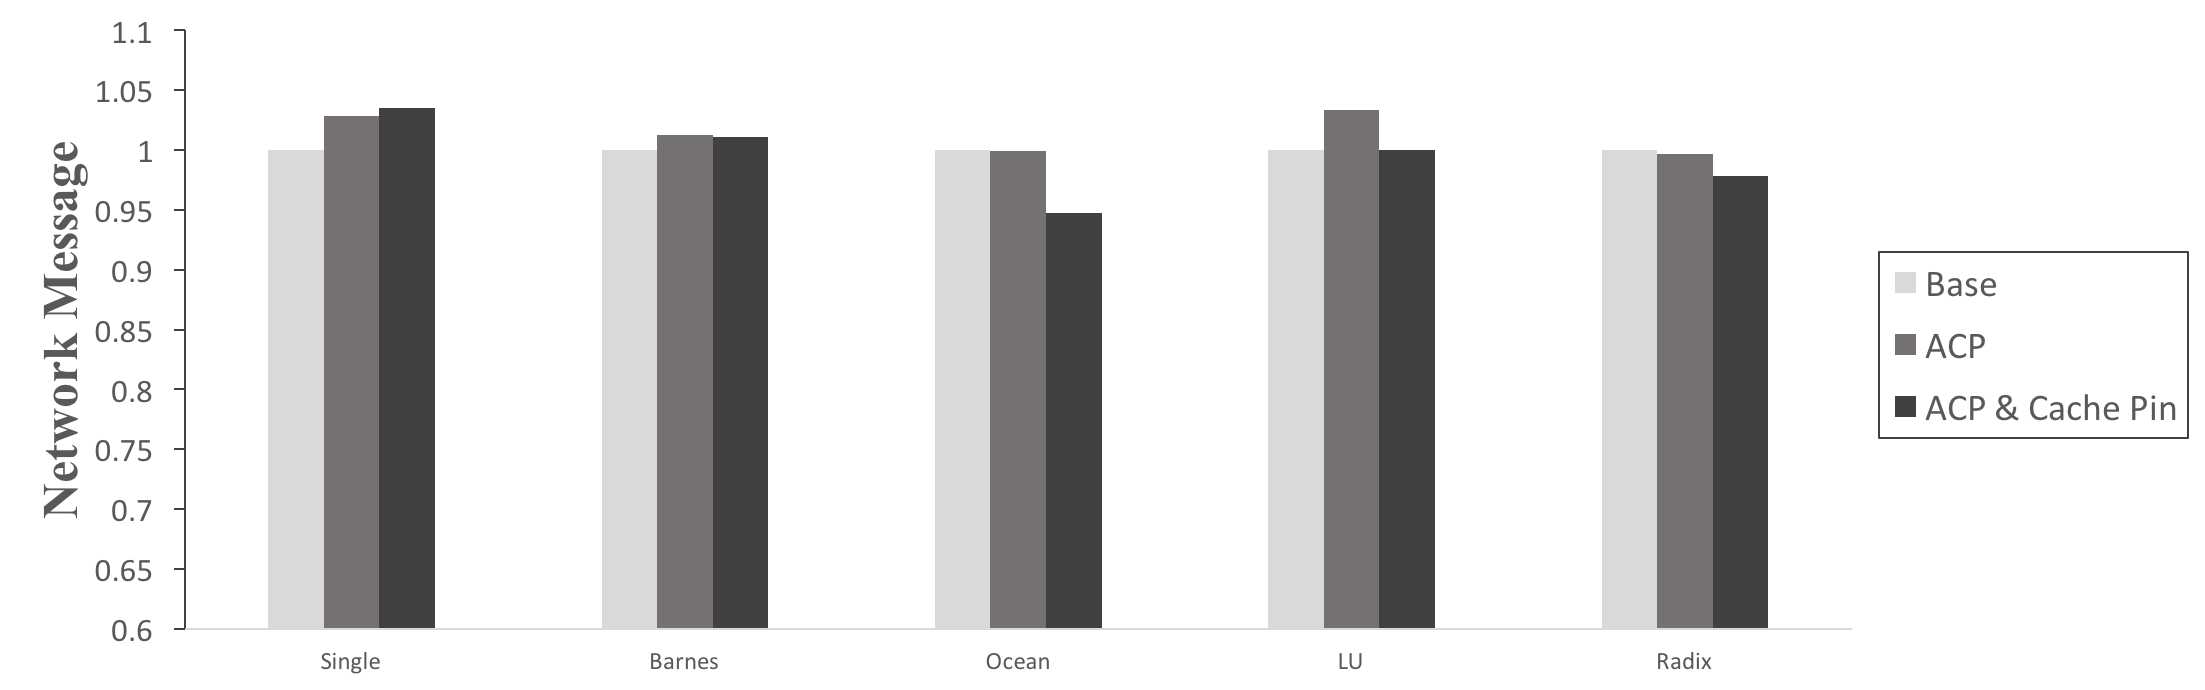
\includegraphics[width=3.5in,height=1.5in]{network_msg.png}
\caption{Network Message}
\label{network_msg}
\end{figure}
\FloatBarrier

\begin{figure}[!h]
\centering
\captionsetup{justification=centering}
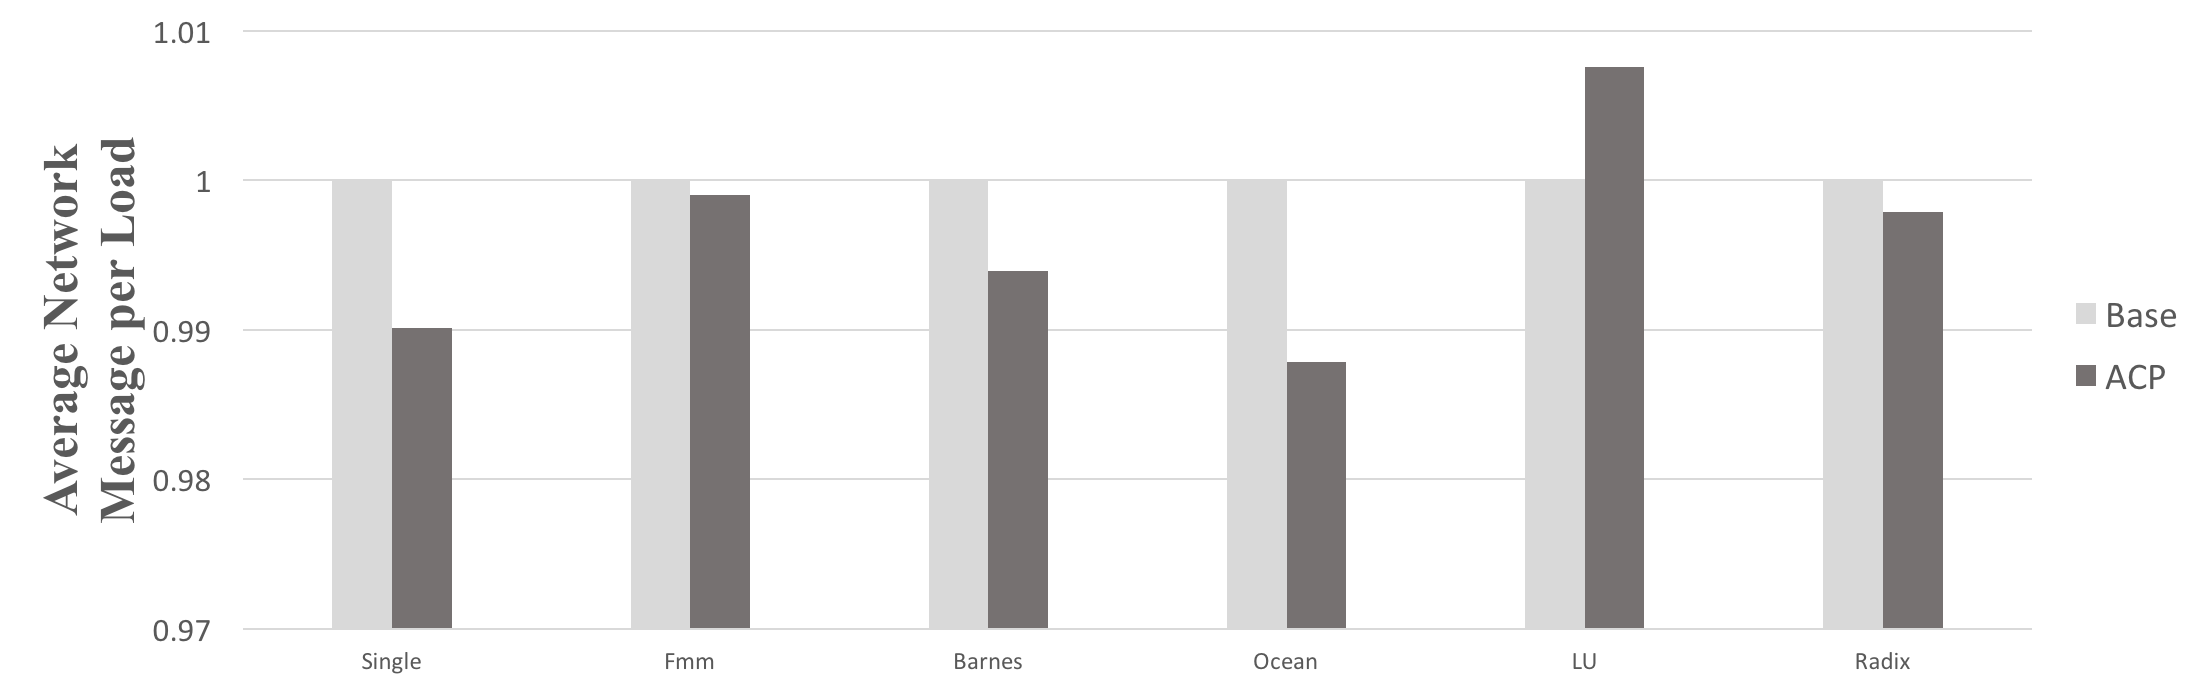
\includegraphics[width=3.5in,height=1.5in]{avg_network_msg_per_load.png}
\caption{Average Network Message per Load}
\label{avg_network_msg_per_load}
\end{figure}
\FloatBarrier

\begin{table}[!h]
\renewcommand{\arraystretch}{2.5}
\caption{Average Network Message Needed to Serve a Load}
\label{table_msg}
\centering
\begin{tabular}{|c|c|c|c|c|c|c|}
\hline
 & Single & Fmm & Barnes & Ocean & LU & Radix \\
\hline
Base & 2.215 & 1.447 & 1.417 & 1.497 & 1.378 & 1.504 \\
\hline
ACP & 2.193 & 1.445 & 1.408 & 1.479 & 1.388 & 1.501 \\
\hline
\end{tabular}
\end{table}
\FloatBarrier

\subsubsection{Write-back Delegation}
As introduced in Section 4, we delegate the write-back responsibility to either producer or consumer depending on different situations. Consumer does not need to issue write-back on cache eviction because producer will keeping modifying shared data and forwarding to consumers. By delegating write-back responsibility to producer on cache eviction, we reduce network message and eviction overhead.

\newpage

\begin{figure}[!h]
\centering
\hfil
\captionsetup{justification=centering}
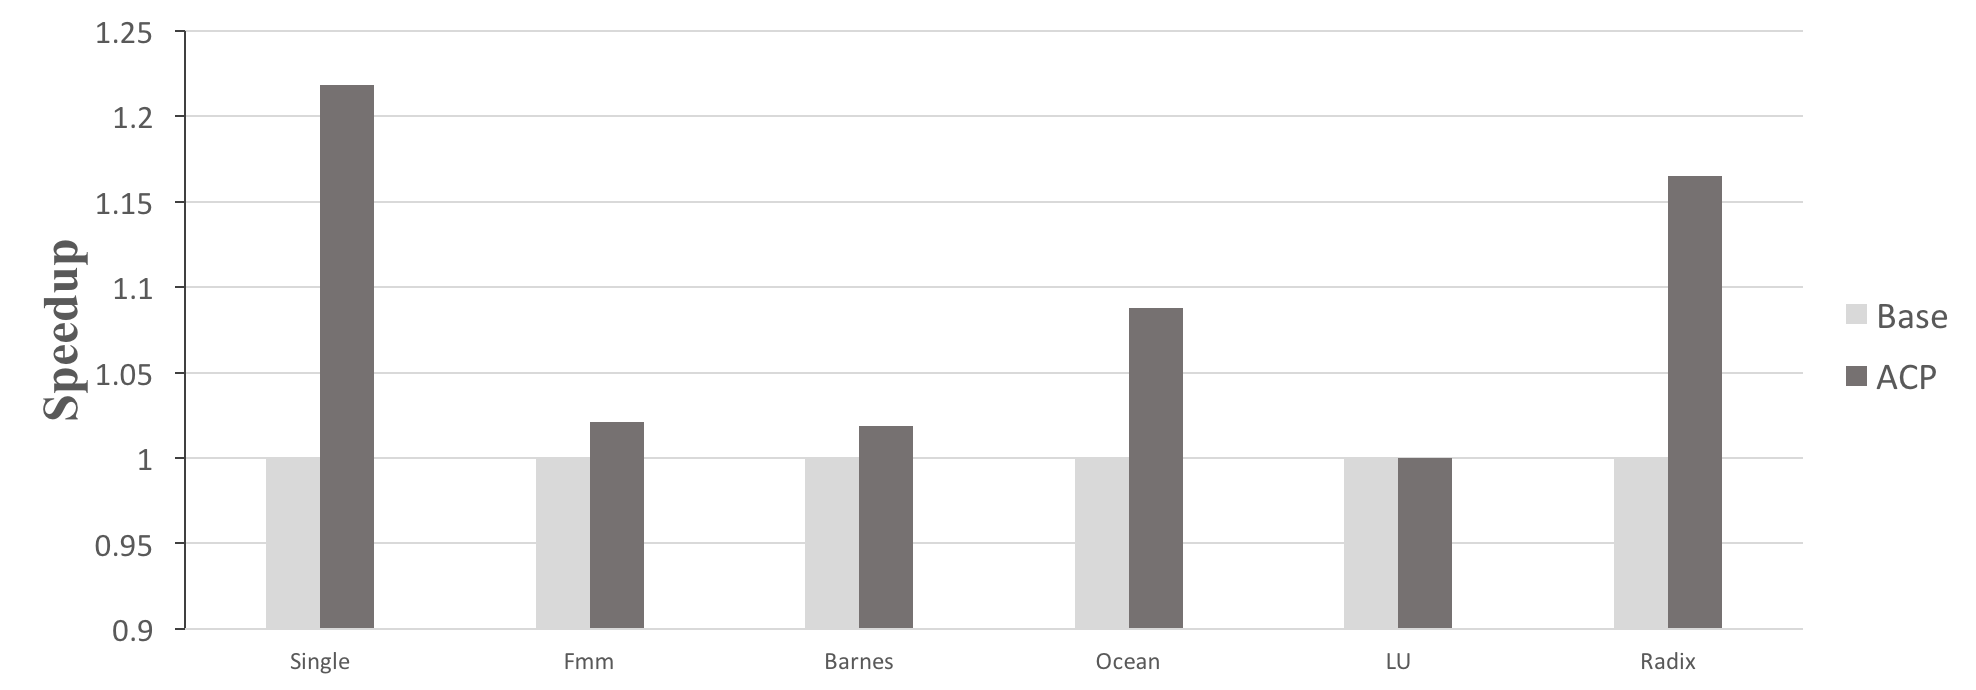
\includegraphics[width=7.5in,height=2.3in]{speedup.png}
\caption{Speedup}
\label{speedup}
\end{figure}
\FloatBarrier

\begin{figure}[!h]
\centering
\captionsetup{justification=centering}
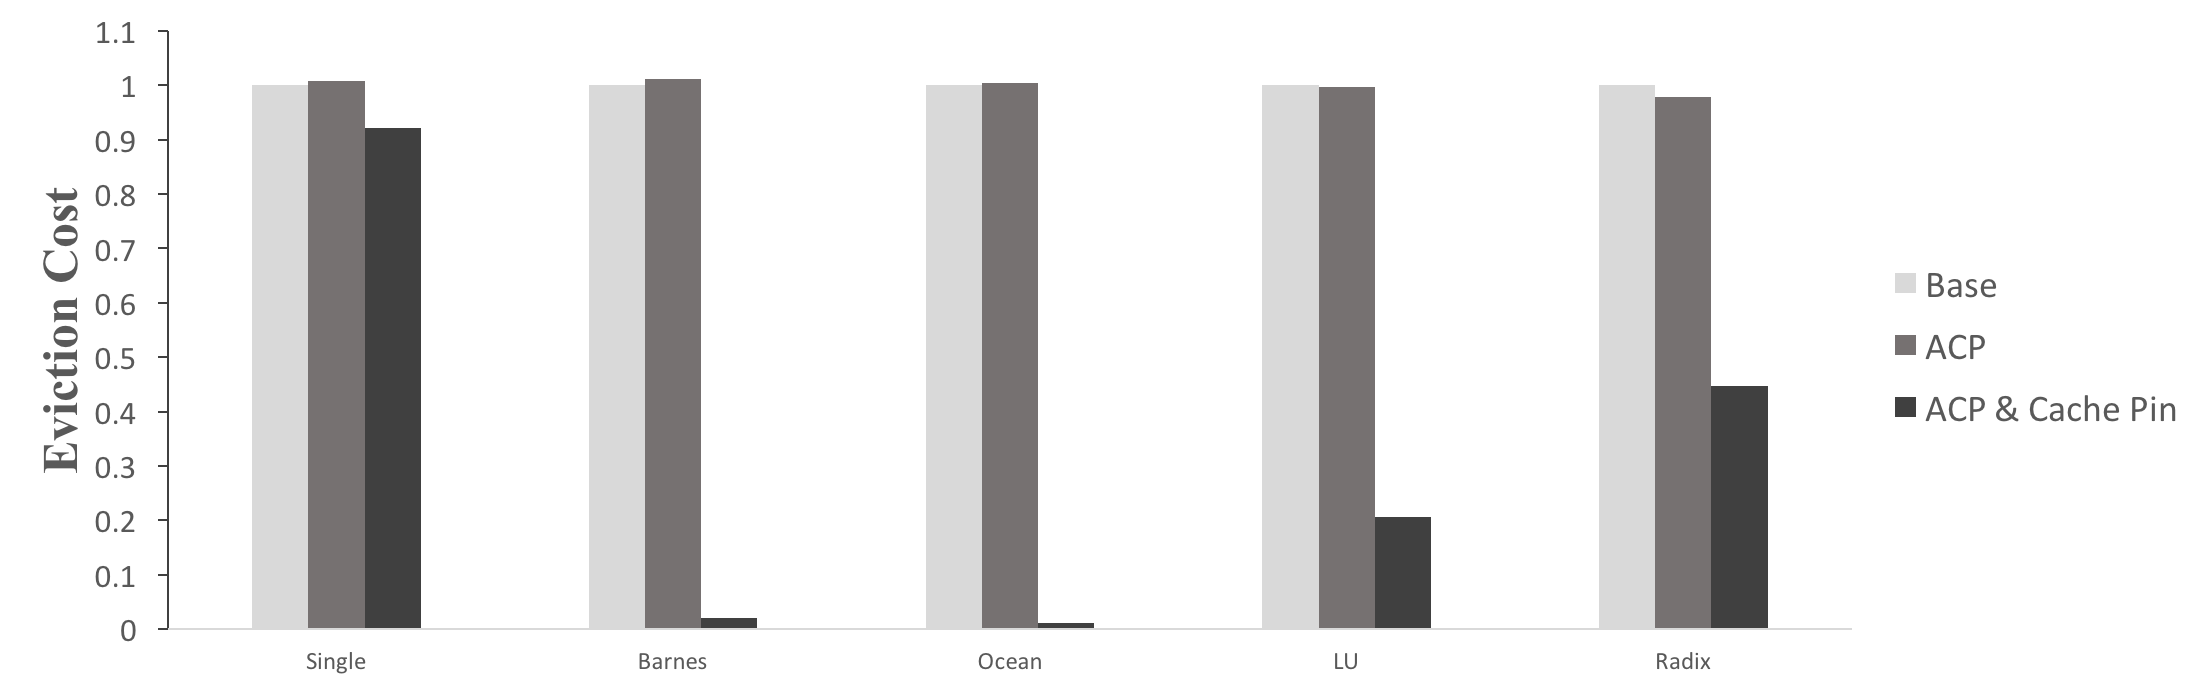
\includegraphics[width=7.5in,height=2.3in]{evict_cycles.png}
\caption{Evict Cycles}
\label{evict_cycles}
\end{figure}
\FloatBarrier

\begin{figure}[!h]
\centering
\captionsetup{justification=centering}
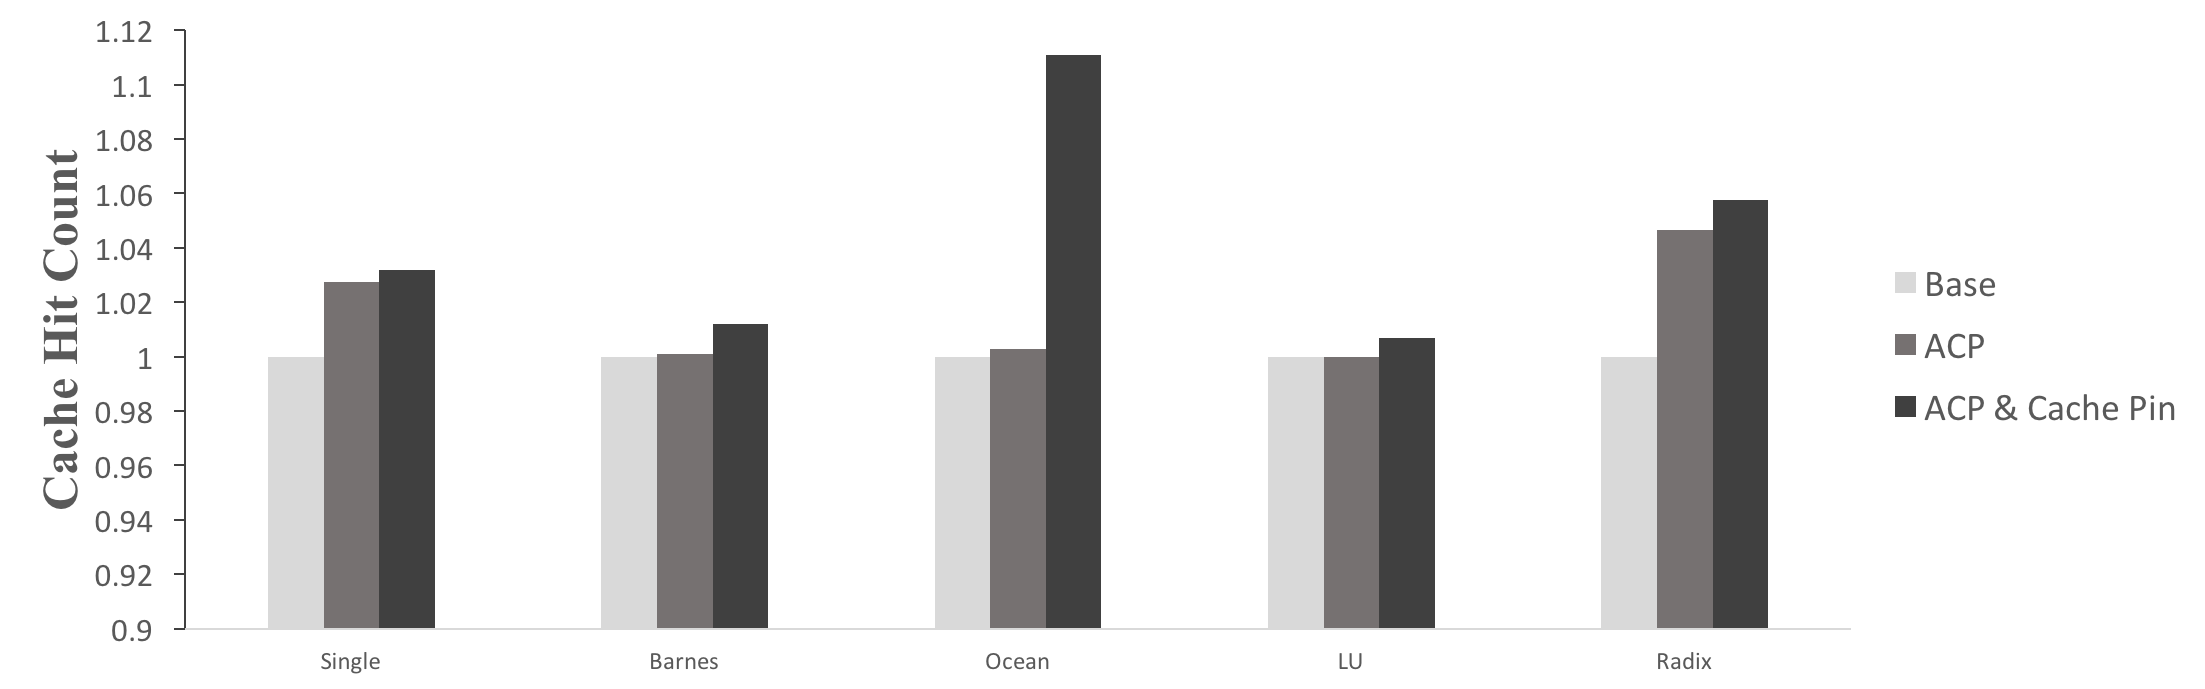
\includegraphics[width=7.5in,height=2.3in]{hit_count.png}
\caption{Hit Count}
\label{hit_count}
\end{figure}
\FloatBarrier


\newpage
\null\newpage

\section{Summary}
In this project, we implement a pintool-based cache simulator that supports multiple cache coherence protocol and offers detailed statistics of cache access behavior. In addition, under the assumption that cache-to-cache communication is physically feasible, we propose an adaptive cache coherence protocol optimized for producer-consumer sharing patterns that intelligently switch from write-invalidate to write-update protocol once stable producer-consumer sharing is detected. We evaluate the adaptive protocol on applications with varying degree of producer-consumer sharing patterns. As a result, the proposed adaptive protocol achieves noticeable speedup with very little network traffic overhead.


\section{Future Works}

Pintool-based \cite{pintool} cache simulator offers a fine-grained investigation of cache access behavior but it comes with a cost --- the observation might deviates from the actual behavior due to the extra instructions instrumented by pintool. So one of the future works is to equip the cache simulator with functionalities that can synchronize application threads so as to observe more accurate cache access events to mitigate the effect of pintool instrumentation. In addition, we assume that directory banks are large enough to hold all line records. We propose in Section 4 that when directory lines are evicted, the extra bits for detector should be discarded to save memory space. We want to support this feature in the cache simulator.

\begin{thebibliography}{1}

\bibitem{work1}
Cheng, Liqun, John B. Carter, and Donglai Dai. "An adaptive cache coherence protocol optimized for producer-consumer sharing." High Performance Computer Architecture, 2007. HPCA 2007. IEEE 13th International Symposium on. IEEE, 2007.

\bibitem{nbody}
Singh, J. P.  Parallel Hierarchical N-body Methods and Their Implications for Multiprocessors.  PhD Thesis, Stanford University, February 1993.

\bibitem{barnes}
Holt, C. and Singh, J. P.  Hierarchical N-Body Methods on Shared Address Space Multiprocessors.  SIAM Conference on Parallel Processing for Scientific Computing, Feb 1995, to appear.

\bibitem{ocean}
Brandt, A. Multi-Level Adaptive Solutions to Boundary-Value Problems. Mathematics of Computation, 31(138):333-390, April 1977.

\bibitem{lu}
Woo, S. C., Singh, J. P., and Hennessy, J. L.  The Performance Advantages of Integrating Block Data Transfer in Cache-Coherent Multiprocessors. Proceedings of the 6th International Conference on Architectural Support for Programming Languages and Operating Systems (ASPLOS-VI), October 1994.

\bibitem{wiki}
https://en.wikipedia.org/wiki/Producer-–consumer\_problem

\bibitem{nbody_wiki}
https://en.wikipedia.org/wiki/N--body\_problem

\bibitem{splash}
http://www.capsl.udel.edu/splash/

\bibitem{pintool}
https://software.intel.com/sites/landingpage/pintool/docs/76991/Pin/html/

\end{thebibliography}

\end{document}
